\section{Classical Multi-Party Computation}

\begin{refsection}

\subsection{Introduction}
Multi-Party Computation (MPC), also known as Secure Function Evaluation, allows two or more parties
to correctly compute a function of their private inputs without exposure, i.e., without
the input of one party being revealed to the other parties.
In other terms, a generic function \textit{f} receives as input a set $\{a_1,a_2,\dots,a_n\}$
of arguments, where $a_i$ is the input of the i-th party, and $1\leq i\leq n$, and outputs a value \textit{c}, which represents the result
of the joint computation of \textit{f}, as shown in Figure \ref{fig:mpcscheme}.
The output of \textit{f} is given by the following expression.
\begin{equation}\label{eq:mpc}
c = f(a_1,a_2,\dots,a_n)
\end{equation}

\renewcommand{\figurename}{Figure}
\begin{figure}[H]
\centering
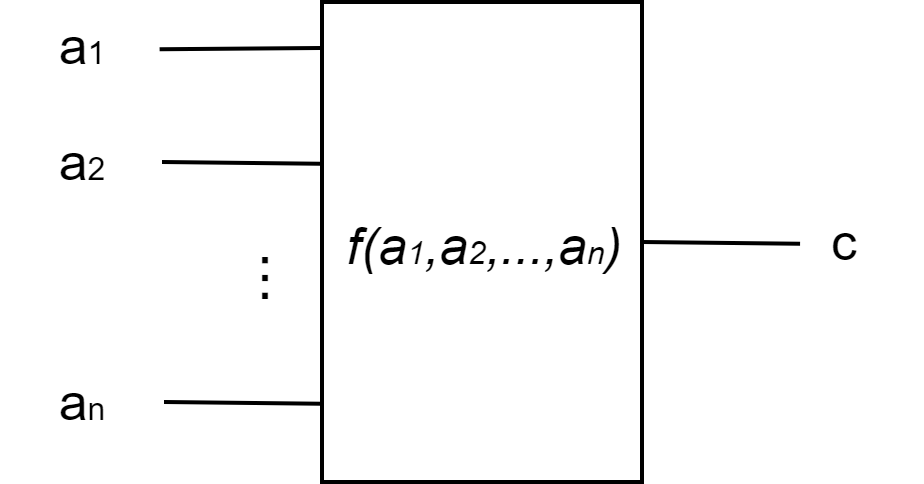
\includegraphics[width=.4\linewidth]{./sdf/classical_mpc/figures/mpc_scheme}
\caption{Multi-Party Computation Diagram}
\label{fig:mpcscheme}
\end{figure}

There are two main models in the literature for the analysis of the Multi-Party Computation problems. The ideal model, which consists in using a Trusted Third Party (TTP). The parties provide their input to the TTP, who will perform the computation of the function. The result is then sent to all the parties. This paradigm relies on the trustworthiness of the TTP because if it turns corrupt, it can supply the private input of one party to the others. This model is extensively used due to its easy implementation and protocols available which prevent the TTP from acting maliciously. The real model of MPC does not use a TTP. In this model, the parties agree on some protocol which will allow them to jointly compute the function. Different protocols are needed for different MPC models and different party behavior models. In \ref{mpcproblemsandsolutions} we will be analyzing different solutions to known MPC problems.

\renewcommand{\figurename}{Figure}
\begin{figure}[H]
\centering
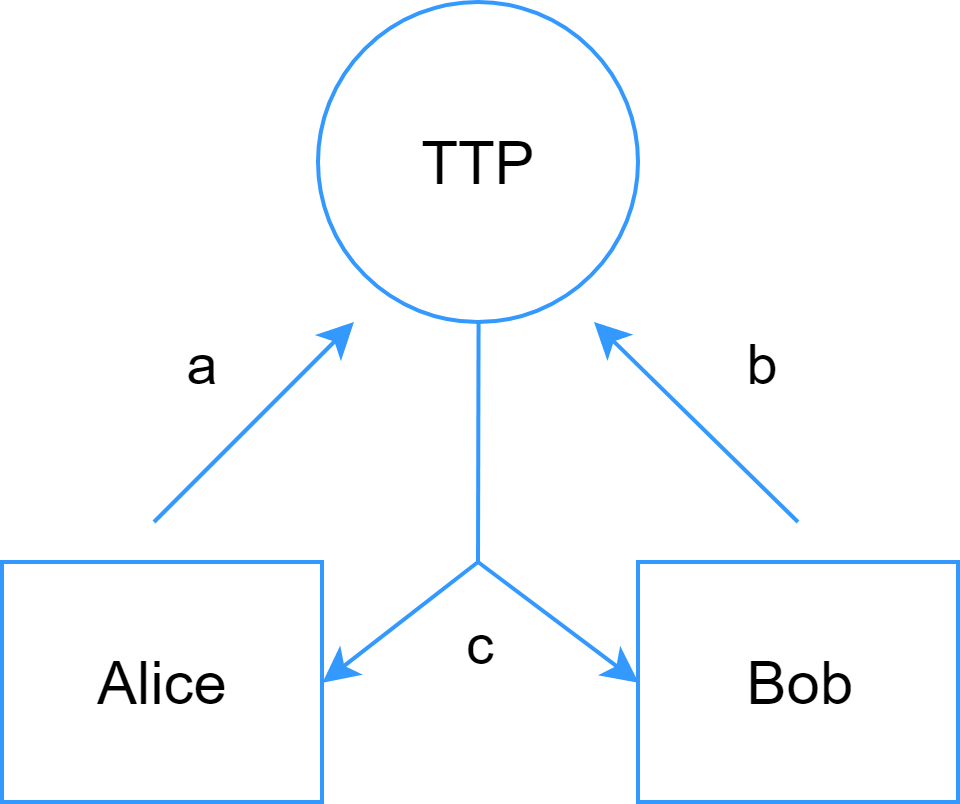
\includegraphics[width=.3\linewidth]{./sdf/classical_mpc/figures/ttp_scheme}
\caption{MPC using a Third Trusted Party}
\label{fig:ttpscheme}
\end{figure}

\subsection{Two-Party Computation}
Two-Party Computation (2PC) is a specific case of MPC, where a generic function \textit{f} receives as input a set $\{a,b\}$
of arguments, where \textit{a} is the input from the first party and \textit{b} is the input from the second,
and outputs a value \textit{c}, as shown in Figure \ref{fig:tpcscheme}.
The output of \textit{f} is given by the following expression.
\begin{equation}\label{eq:tpc}
c = f(a,b)
\end{equation}

\renewcommand{\figurename}{Figure}
\begin{figure}[H]
\centering
\includegraphics[width=.4\linewidth]{./sdf/classical_mpc/figures/two_party_computation_scheme}
\caption{Two-Party Computation Diagram}
\label{fig:tpcscheme}
\end{figure}

\subsection{Party Behavior Models}
There are three main models to describe the behavior of a party. The honest model, where the party follows the protocol and respects the privacy of other parties. A semi honest model, where the party follows the protocol but also tries to gain additional information other than the result. The corrupt model, where the party neither follows the protocol nor respects the privacy of other parties.

\pagebreak

\subsection{MPC Problems and Solutions}\label{mpcproblemsandsolutions}
In this subsection, we will be analyzing different solutions to known MPC problems without the presence of a TTP. We will present a problem and then analyze various solution.

\subsubsection{The Millionaires' Problem}
Consider 2 parties, Alice and Bob, with inputs $a$ and $b$ respectively. The output of this function is $1$ when $a < b$
and $0$ when $a \geq b$. In other terms,
\[
f(a,b) = \left \{
          \begin{tabular}{ccc}
          0, if $a \geq b$ \\
          1, if $a < b$
          \end{tabular}
        \right.
\]
%%%%%%%%%%%%%%%%%%%%%%%%%%%% Solutions Millionaires' Problem %%%%%%%%%%%%%%%%%%%%%%%%%%%%
\paragraph{Yao's Solution}
This method was proposed by Andrew C. Yao in 1982 \cite{yao1982}. Let $E_a$ be Alice's public key, $E_a(x)$ the process of encrypting input $x$ by performing
a bitwise XOR between $x$ and Alice's public key and $D_a(x)$ the process of decrypting input x.
For this example, we will assume the following values: $a = 7$, $b = 3$, $N = 16$, $x = 39226$, $p = 211$ and $E_a = 24698$.

\begin{enumerate}
\item Bob picks a random N-bit integer, $x$, and computes privately the value of $E_a(x)$; calls the result k.
\begin{equation}\label{eq:encryptingX}
k = E_a(x) = x \oplus E_a = 63808
\end{equation}

\item Bob sends Alice the number $k - b + 1$
\begin{equation}\label{eq:encryptingX}
k - b + 1 = 63806
\end{equation}

\item Alice computes privately the values of $Y_u = D_a(k - b + u)$ for $u = 1,2,\ldots,10$\\
\[
Y_u = \begin{bmatrix}
        39236,&39237,&39226,&39227,&39224,&39225,&39230,&39231,&39228,&39229
      \end{bmatrix}
\]

\item Alice generates a random prime $p$ of $N/2$ bits, and computes $Z_u = Y_u$  mod  $p$
\[
Z_u = \begin{bmatrix}
        201,&202,&191,&192,&189,&190,&195,&196,&193,&194
      \end{bmatrix}
\]

\item Alice sends the prime $p$ and the following 10 numbers to Bob: $Z_1,Z_2,\ldots,Z_a$
followed by $Z_{a+1}+1,\ldots,Z_{10}+1$
\[
M = \begin{bmatrix}
        201,&202,&191,&192,&189,&190,&195,&197,&194,&195
      \end{bmatrix}
\]
Note that only the elements of $Z_u$ and $M$ with indexes 7, 8, 9 and 10 are different, since $a = 7$

\item Bob looks at the b-th number sent by Alice, and decides that $a \geq b$ if it is equal to $x$ mod $p$,
and $a < b$ otherwise. In other terms,
\[
f(a,b) = \left \{
          \begin{tabular}{ccc}
          0, if $M_b = x$ mod $p$ \\
          1, if $M_b \ne x$ mod $p$
          \end{tabular}
        \right.
\]
Since $M_b = x$ mod $p = 191$, we have $f(a,b) = 0$, which means that $a \geq b$.
\end{enumerate}
%%%%%%%%%%%%%%%%%%%%%%%%%%%%%%%%%%%%%%%%%%%%%%%%%%%%%%%%%%%%%%%%%%%%%%%%%%%%%%%%%%%%%%%%%%

\subsubsection{1-2 Oblivious Transfer}
Consider 2 parties, Alice and Bob. Alice has a set of messages $A=\{m_0,m_1,m_2,\ldots,m_{n-1}\}$
and Bob has an index $b$. The output of this function should be $m_b$, i.e., the message from Alice's set of index $b$. Bob should not gain any more information other than $m_b$ and Alice should not know the value of $b$.
\begin{equation}\label{eq:messageaccess}
f(A,b) = A_b
\end{equation}

<<<<<<< HEAD
\renewcommand{\figurename}{Figure}
\begin{figure}[H]
\centering
\includegraphics[width=.4\linewidth]{./sdf/classical_mpc/figures/OT}
\caption{Oblivious Transfer Diagram}
\label{fig:otscheme}
\end{figure}

%%%%%%%%%%%%%%%%%%%%%%%%%%%% Solutions 1-2 Oblivious Transfer %%%%%%%%%%%%%%%%%%%%%%%%%%%%



%%%%%%%%%%%%%%%%%%%%%%%%%%%%%%%%%%%%%%%%%%%%%%%%%%%%%%%%%%%%%%%%%%%%%%%%%%%%%%%%%%%%%%%%%%

\subsubsection{Average Value}
Consider 2 parties, Alice and Bob, with inputs $a$ and $b$ respectively. The output of this function should be the average value of $a$ and $b$
. In other terms,
\begin{equation}\label{eq:tpc}
f(a,b) = \frac{a+b}{2}
\end{equation}
=======
\subsubsection{Average Value}
%Complete this section


>>>>>>> Goncalo

%%%%%%%%%%%%%%%%%%%%%%%%%%%%% Solutions Average Value %%%%%%%%%%%%%%%%%%%%%%%%%%%%%%%%%%


%%%%%%%%%%%%%%%%%%%%%%%%%%%%%%%%%%%%%%%%%%%%%%%%%%%%%%%%%%%%%%%%%%%%%%%%%%%%%%%%%%%%%%%%%%
\subsection{Garbled Circuit Protocol}
Introduced in 1986 by Andrew Yao, the Garbled Circuit protocol (GC) addresses the case
of Two-Party Computation (2PC), without the presence of a trusted third party.
GC allows a secure evaluation of a function given as a Boolean circuit that is represented as a series of logic gates.
The circuit is known to both parties.\\

\subsection{Hardware Description Languages}
Contrary to Programming Languages such as C or C++, which are used to specify a set of instructions to a computer, Hardware Description Languages (HDL) are computer languages used to describe the structure and behavior of digital logic circuits. They allow for the synthesis of HDL description code into a netlist (specification of physical eletronic components, such as AND gates or NOT gates, and how they are connected together).

\subsection{TinyGarble}
TinyGarble is a GC framework that takes advantage of powerful logic synthesis techniques, provided by both HDL synthesis tools
and TinyGarble's custom libraries, in order improve the overall efficiency of the GC protocol.
It it possible to describe the circuit using High-Level Programming Languages (HLPL) such as C, although High-Level Synthesis (HLS) is required. HLS is performed by High-Level Synthesis tools, such as SPARK for the C language.

\renewcommand{\figurename}{Figure}
\begin{figure}[H]
\centering
\includegraphics[width=.9\linewidth]{./sdf/classical_mpc/figures/tinygarble_flow_diagram}
\caption{TinyGarble Flow Diagram}
\label{fig:tgdiagram}
\end{figure}

\subsection{ARM2GC}
Although circuit description in HLPL is possible, it is not very efficient when compared to HDL circuit description. ARM2GC addresses this problem, significantly improving the performance of garbled circuits described in HLPL.\\
In the case of 2PC, ARM2GC's approach to GC is based on the ARM processor architecture and consists in providing a public parameter to function \textit{f}, so that its output would be given by the following expression.
\begin{equation}\label{eq:arm2gc}
z = f(a,b,p)
\end{equation}
, where $p$ represents a public parameter, known to both parties.\\
In ARM2GC the Boolean circuit required to perform GC is that of a processor to which the compiled binary of the function is given as a public input ($p$\textit{ = compiled binary of the function}). This optimization is performed by the SkipGate algorithm.



% bibliographic references for the section ----------------------------
\clearpage
\printbibliography[heading=subbibliography]
\end{refsection}
\addcontentsline{toc}{subsection}{Bibliography}
\cleardoublepage
% --------------------------------------------------------------------- 